\section{Parameters identification}

\begin{frame}{Optical sensor characterization}

    \begin{columns}[c, onlytextwidth]

        \begin{column}{0.40\textwidth}

            A mapping between the output voltage of the optical infrared sensor and the position of the ball has been obtained.

        \end{column}

        \begin{column}{0.6\textwidth}

            \begin{figure}[H]
                \centering
                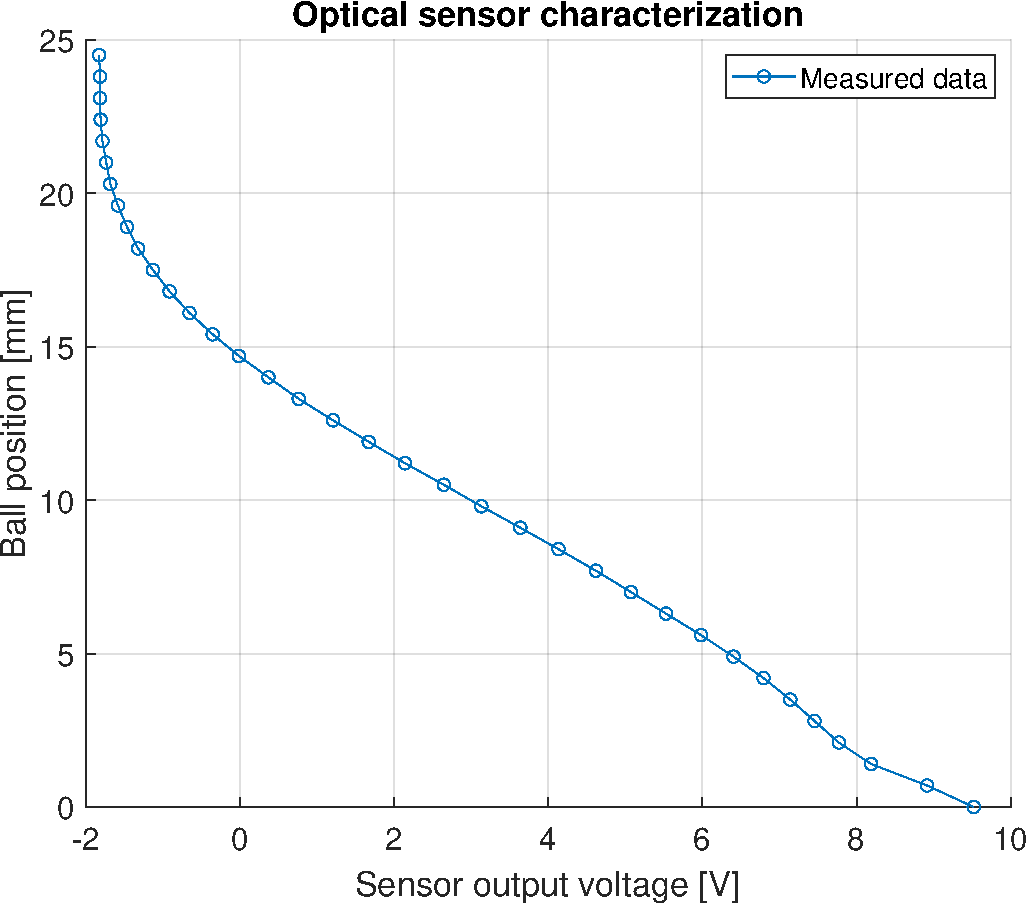
\includegraphics[width=0.8\textwidth]{img/MATLAB/identification/sensor_position.pdf}
                \caption{Ball position as a function of the sensor output voltage}
            \end{figure}

        \end{column}

    \end{columns}

\end{frame}



\begin{frame}{Sensors noise analysis}

    Noises on both the position and current sensors has been analyzed.
    Classical probability indices\footnotemark[1] have been computed to evaluate the quality of the sensors.

    \begin{figure}[H]
        \centering
        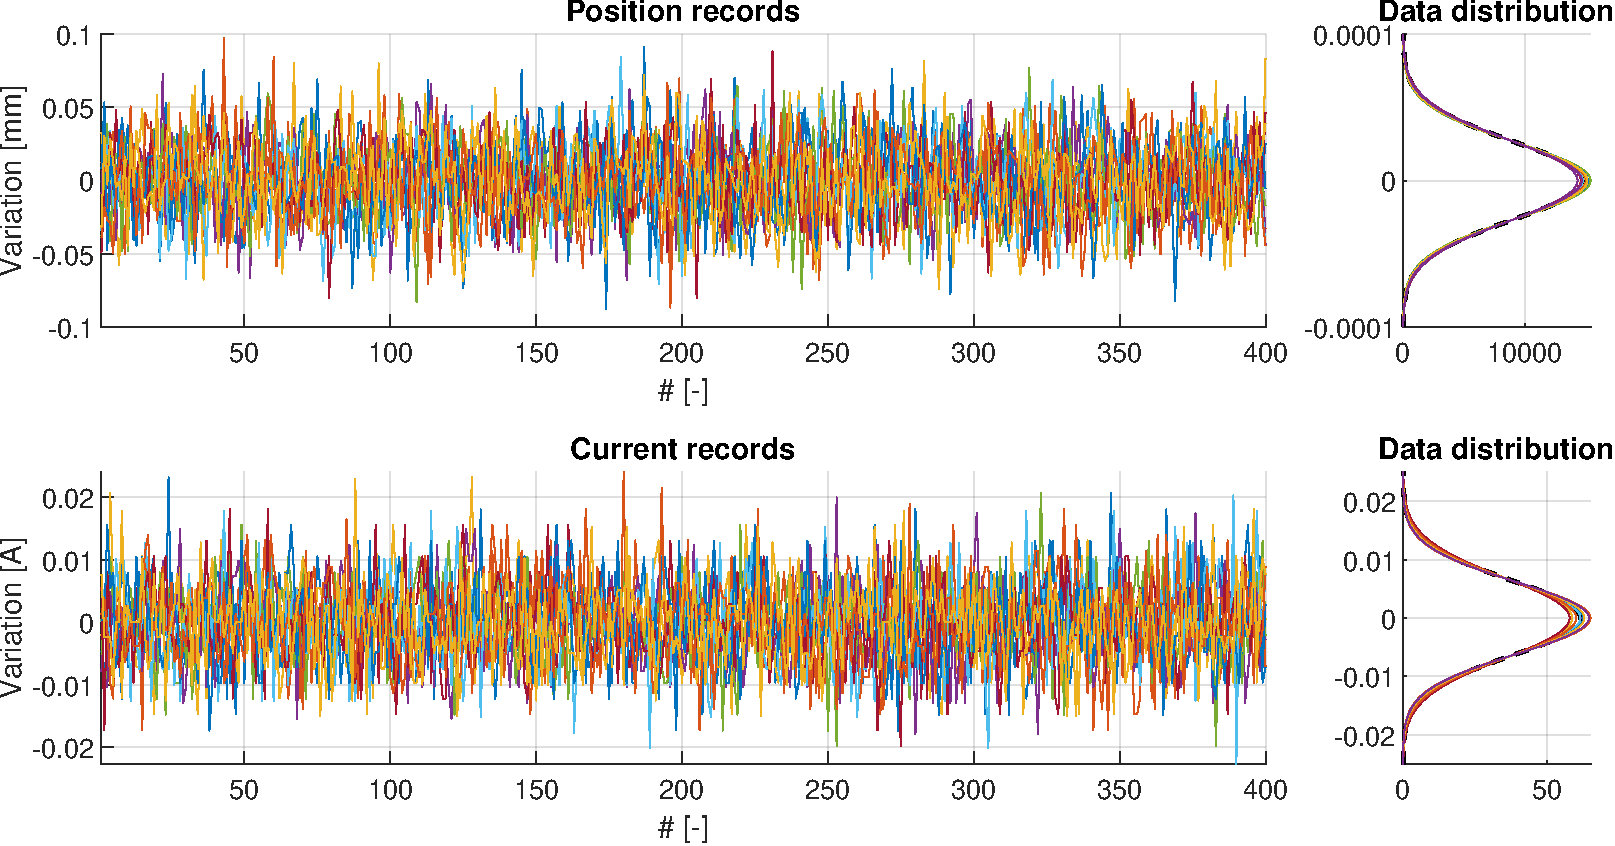
\includegraphics[width=0.9\textwidth]{img/MATLAB/identification/sensor_noises.pdf}
        \caption{Noise analysis for both the position and current sensors}
    \end{figure}

    \footnotetext[1]{Standard deviation and covariance have been considered.}

\end{frame}



\begin{frame}{Control to Voltage mapping}

    \begin{columns}[c, onlytextwidth]

        \begin{column}{0.60\textwidth}

            \begin{figure}
                \centering
                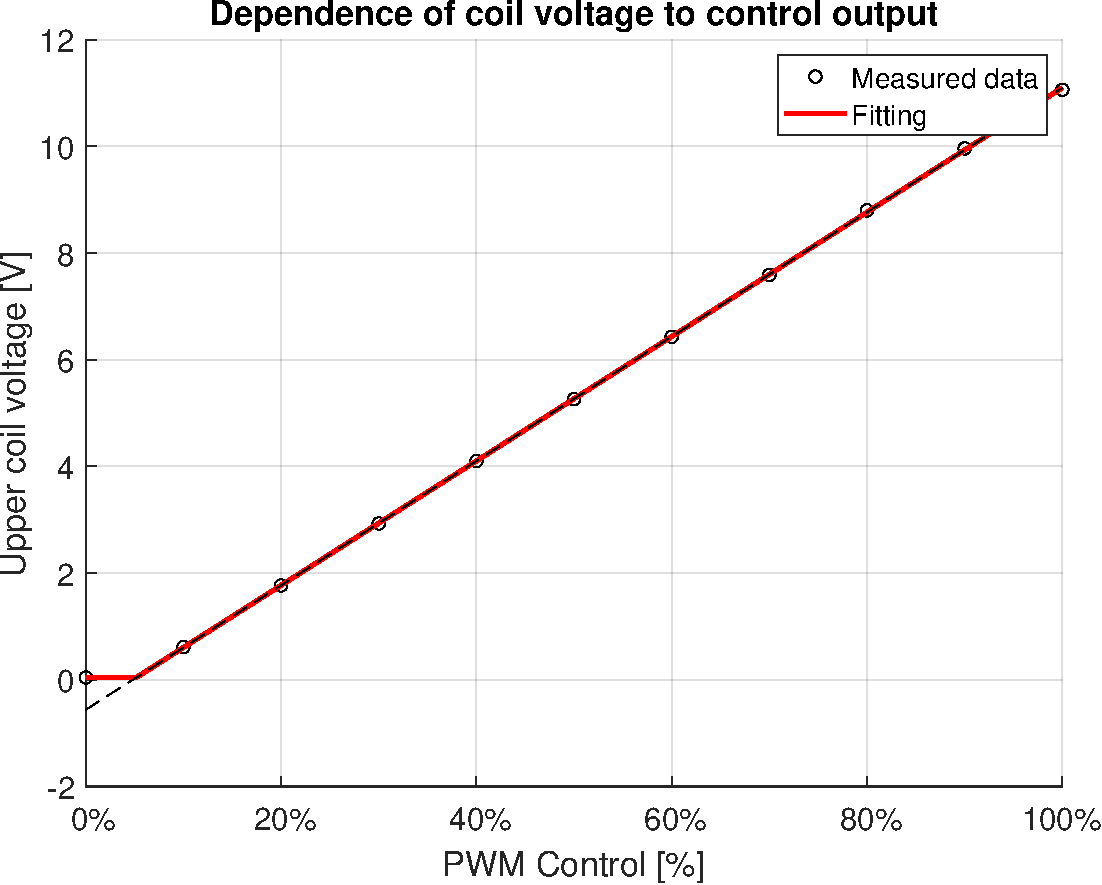
\includegraphics[width=0.8\textwidth]{img/MATLAB/identification/control_to_voltage.pdf}
                \caption{Effective coil voltage $V$ as a function of the control signal $U$}
            \end{figure}

        \end{column}

        \begin{column}{0.40\textwidth}

            Mapping between the control signal $U$ and the effective coil voltage $V$ has also been evaluated.

            \begin{equation}
                V = \begin{cases}
                    V_{min} & \text{if } U < U_{min}    \\
                    k U + c & \text{if } U \geq U_{min}
                \end{cases}
            \end{equation}

        \end{column}

    \end{columns}

\end{frame}



\begin{frame}{Inductance characterization}

    As already discussed, we assume $L(z, I) = L_{0} + L_{z} e^{-a_{z} z} + L_{I} \arctan(a_{I} I - b_{I})$.

    \vspace{9pt}

    \only<1,2>{

        \begin{columns}[c, onlytextwidth]

            \begin{column}{0.40\textwidth}

                Each of the experimental current transients has been fitted with the following RL circuit model:

                \begin{equation}
                    I(t) = \frac{\Delta V}{R_0} \left( 1 - e^{- \frac{R_0}{L(z, I)} t} \right)
                    \label{eq:current_in_rl_circuit}
                \end{equation}

            \end{column}

            \begin{column}{0.60\textwidth}

                \begin{figure}
                    \centering

                    \only<1>{
                        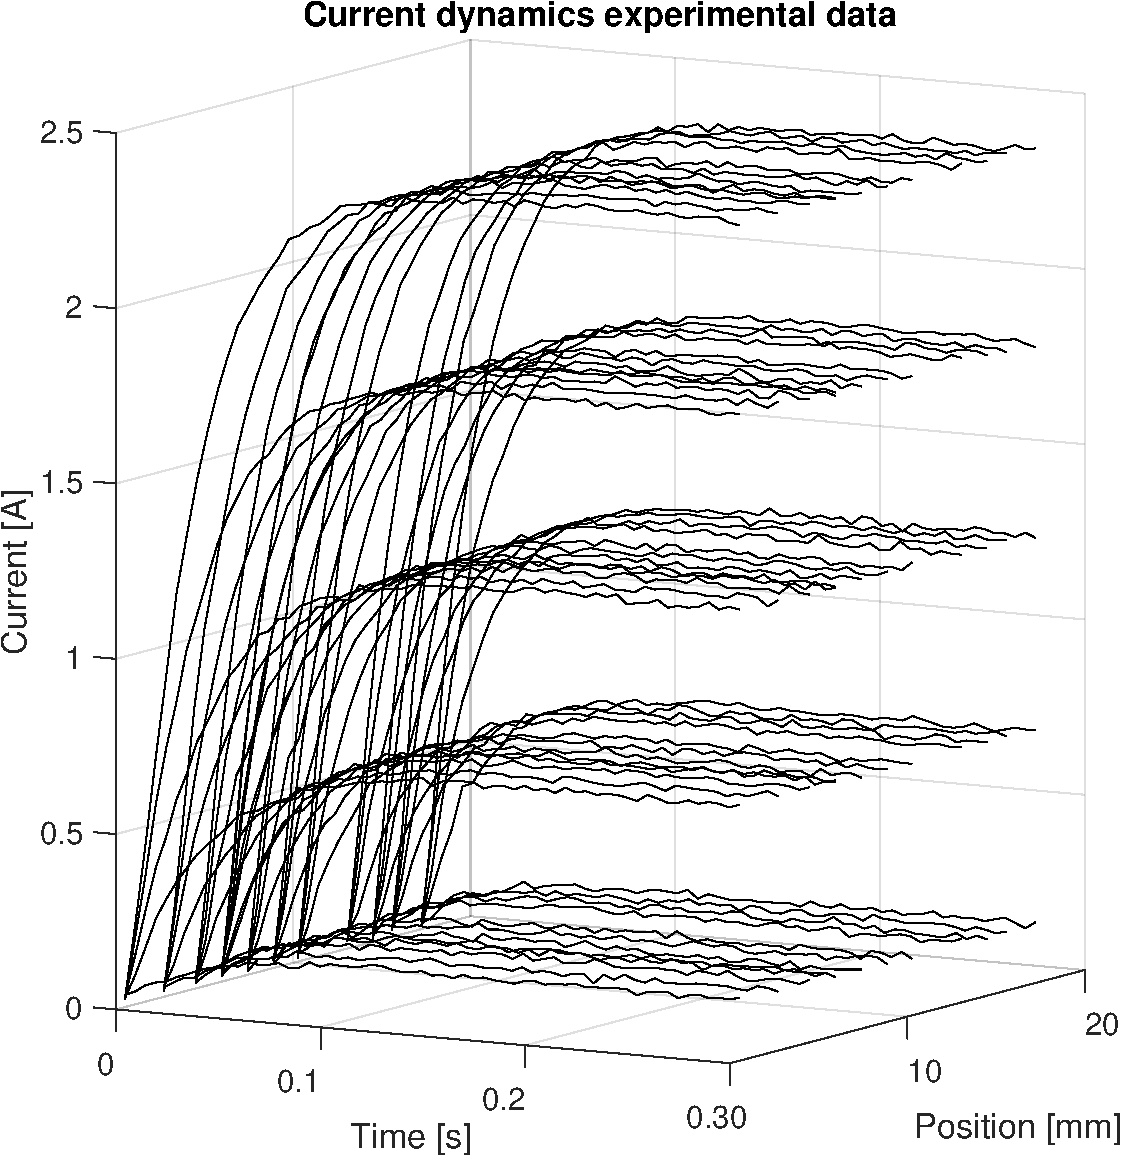
\includegraphics[width=0.8\textwidth]{img/MATLAB/identification/currents_experimental.pdf}
                        \caption{(Some) Experimental current transients for different $z$ (fixed) and $\Delta V$ applied}
                    }

                    \only<2>{
                        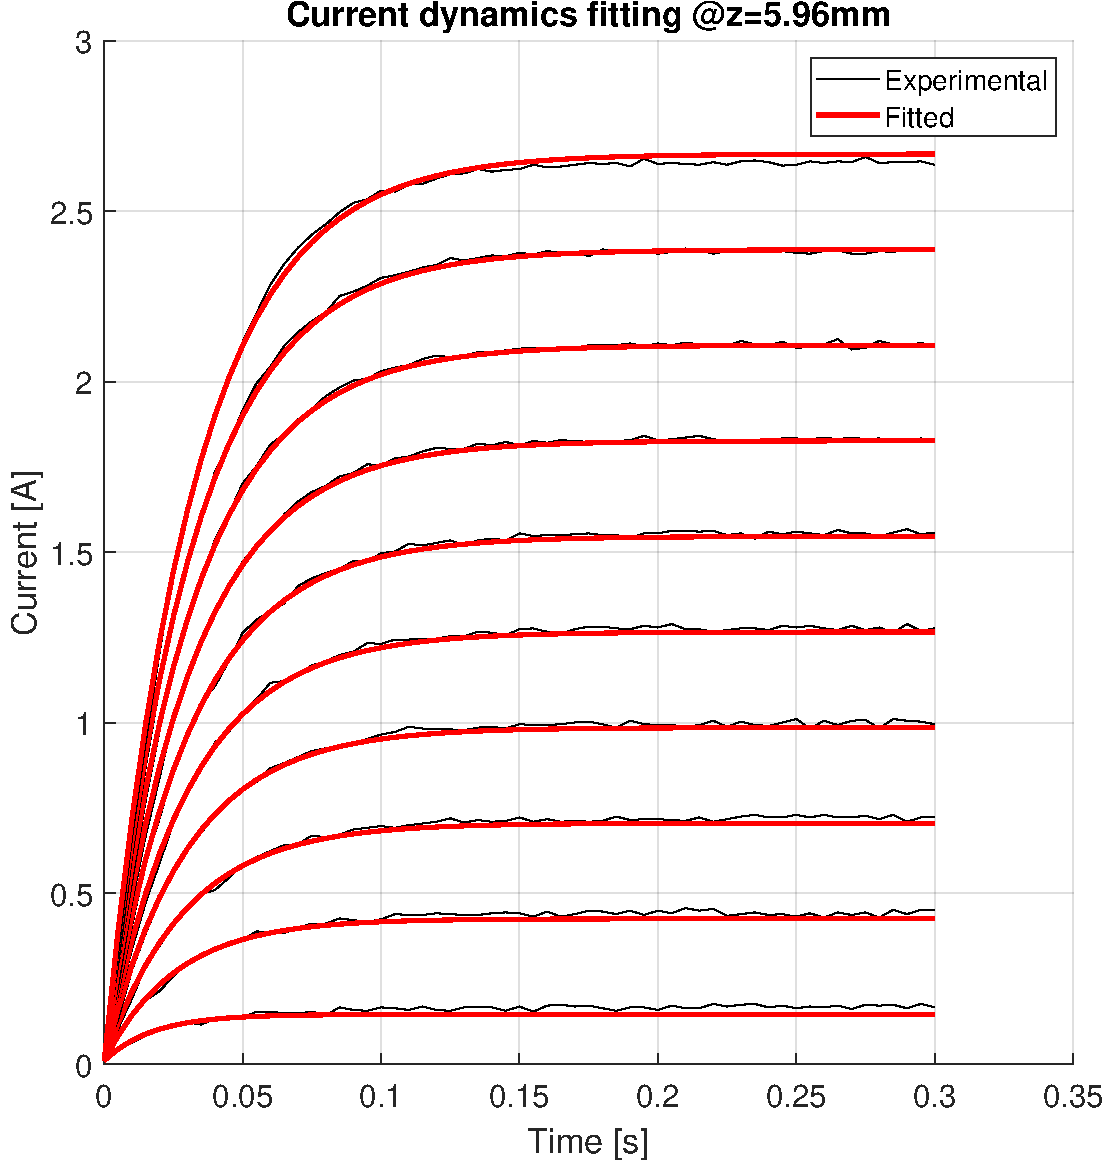
\includegraphics[width=0.8\textwidth]{img/MATLAB/identification/currents_fitted.pdf}
                        \caption{Fitted current transients for a given $z$ (fixed) and different $\Delta V$ applied}
                    }

                \end{figure}

            \end{column}

        \end{columns}

    }

    \only<3>{

        \begin{columns}[c, onlytextwidth]

            \begin{column}{0.40\textwidth}

                Repeating the procedure for many couples of $z$ and $I$, a full model for the inductance is obtained.

                \vspace{9pt}

                In the image, black dots represent the previously computed/fitted values of $L(z, I)$, while the surface represents the complete inductance model.

            \end{column}

            \begin{column}{0.60\textwidth}

                \begin{figure}
                    \centering
                    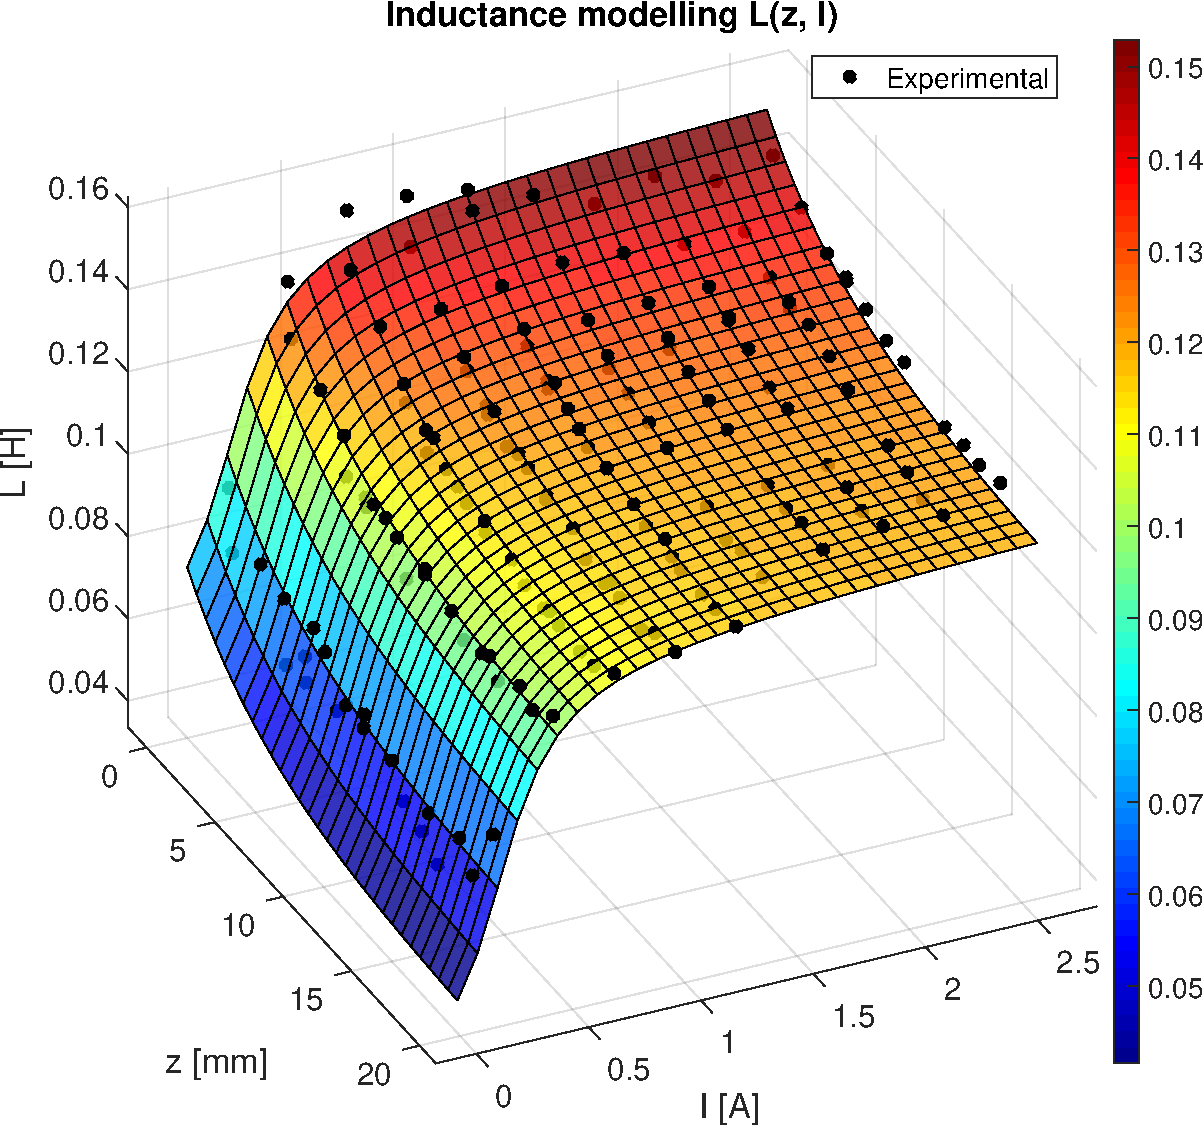
\includegraphics[width=0.85\textwidth]{img/MATLAB/identification/inductance.pdf}
                    \caption{Fitted model for $L(z, I)$}
                \end{figure}
            \end{column}

        \end{columns}

    }

\end{frame}



\begin{frame}{Electromagnetic force analysis}

    \only<1>{

        \vspace{9pt}

        \begin{columns}[c, onlytextwidth]

            \begin{column}{0.60\textwidth}

                \begin{figure}
                    \centering
                    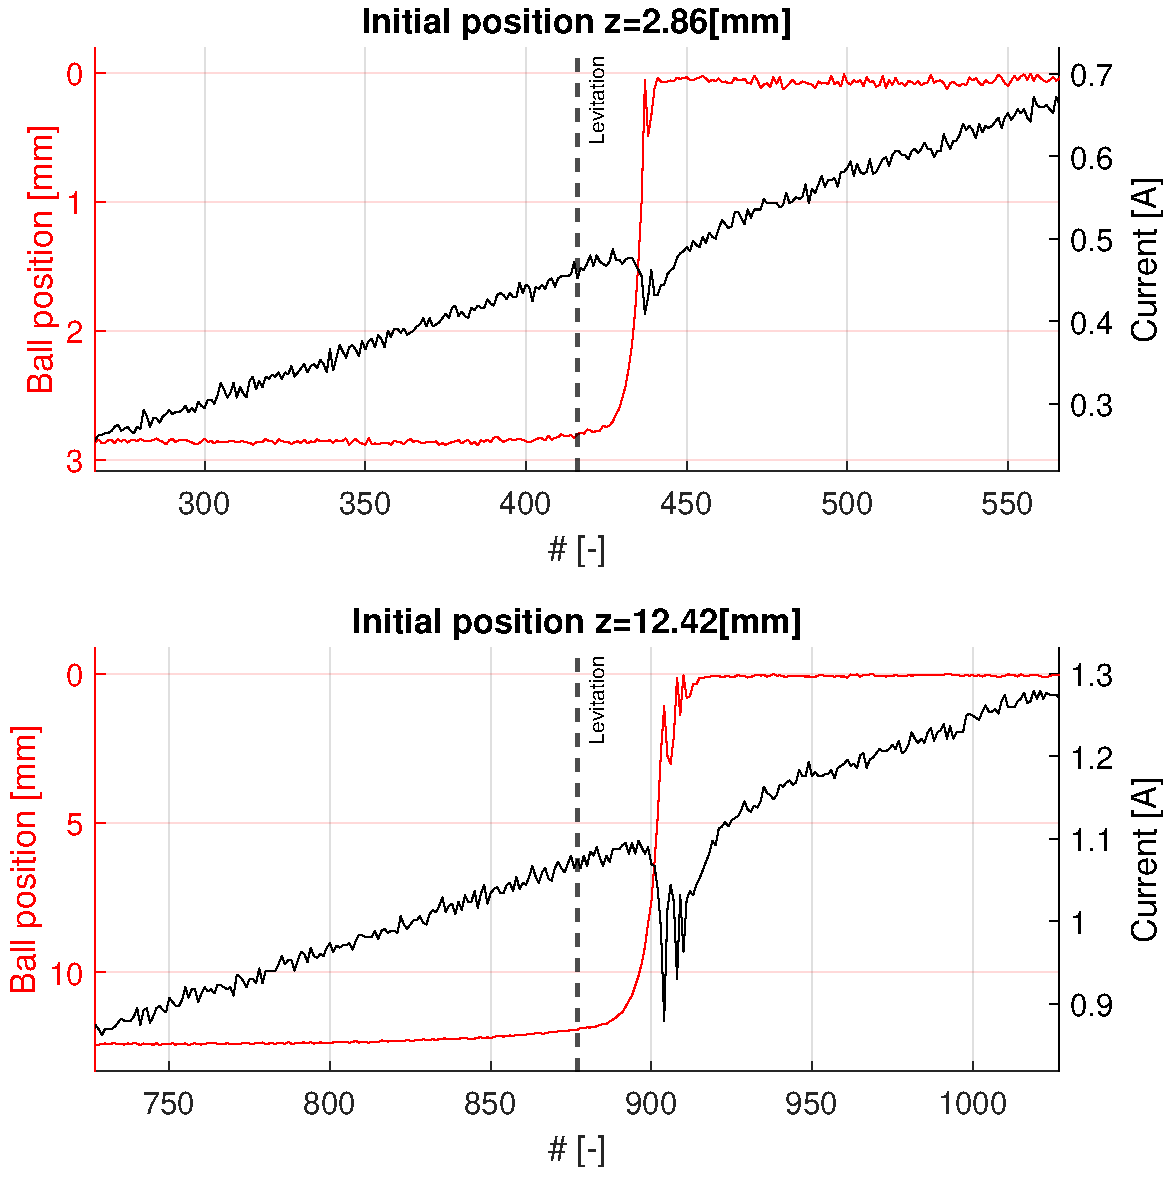
\includegraphics[width=0.85\textwidth]{img/MATLAB/identification/currents_for_force-cropped.pdf}
                    \caption{Current and ball position around the incipient point}
                \end{figure}

            \end{column}

            \begin{column}{0.40\textwidth}

                From the equations of motion, we have found $F_{em} = \frac{1}{2} \frac{\partial L}{\partial z} I^2$.

                \vspace{9pt}

                Knowing that at the incipient $F_{em} = mg$, we can compute $\frac{\partial L}{\partial z}$ to observe if it's consistent with the previously obtained parameters.

                \begin{equation}
                    \left(\frac{\partial L}{\partial z} = \frac{2mg}{I^2}\right)\Big|_{\text{incipient}}
                \end{equation}

            \end{column}

        \end{columns}

    }

    \only<2>{

        Force analysis confirmed the validity of the parameters already identified for the inductance model.

        \begin{figure}
            \centering
            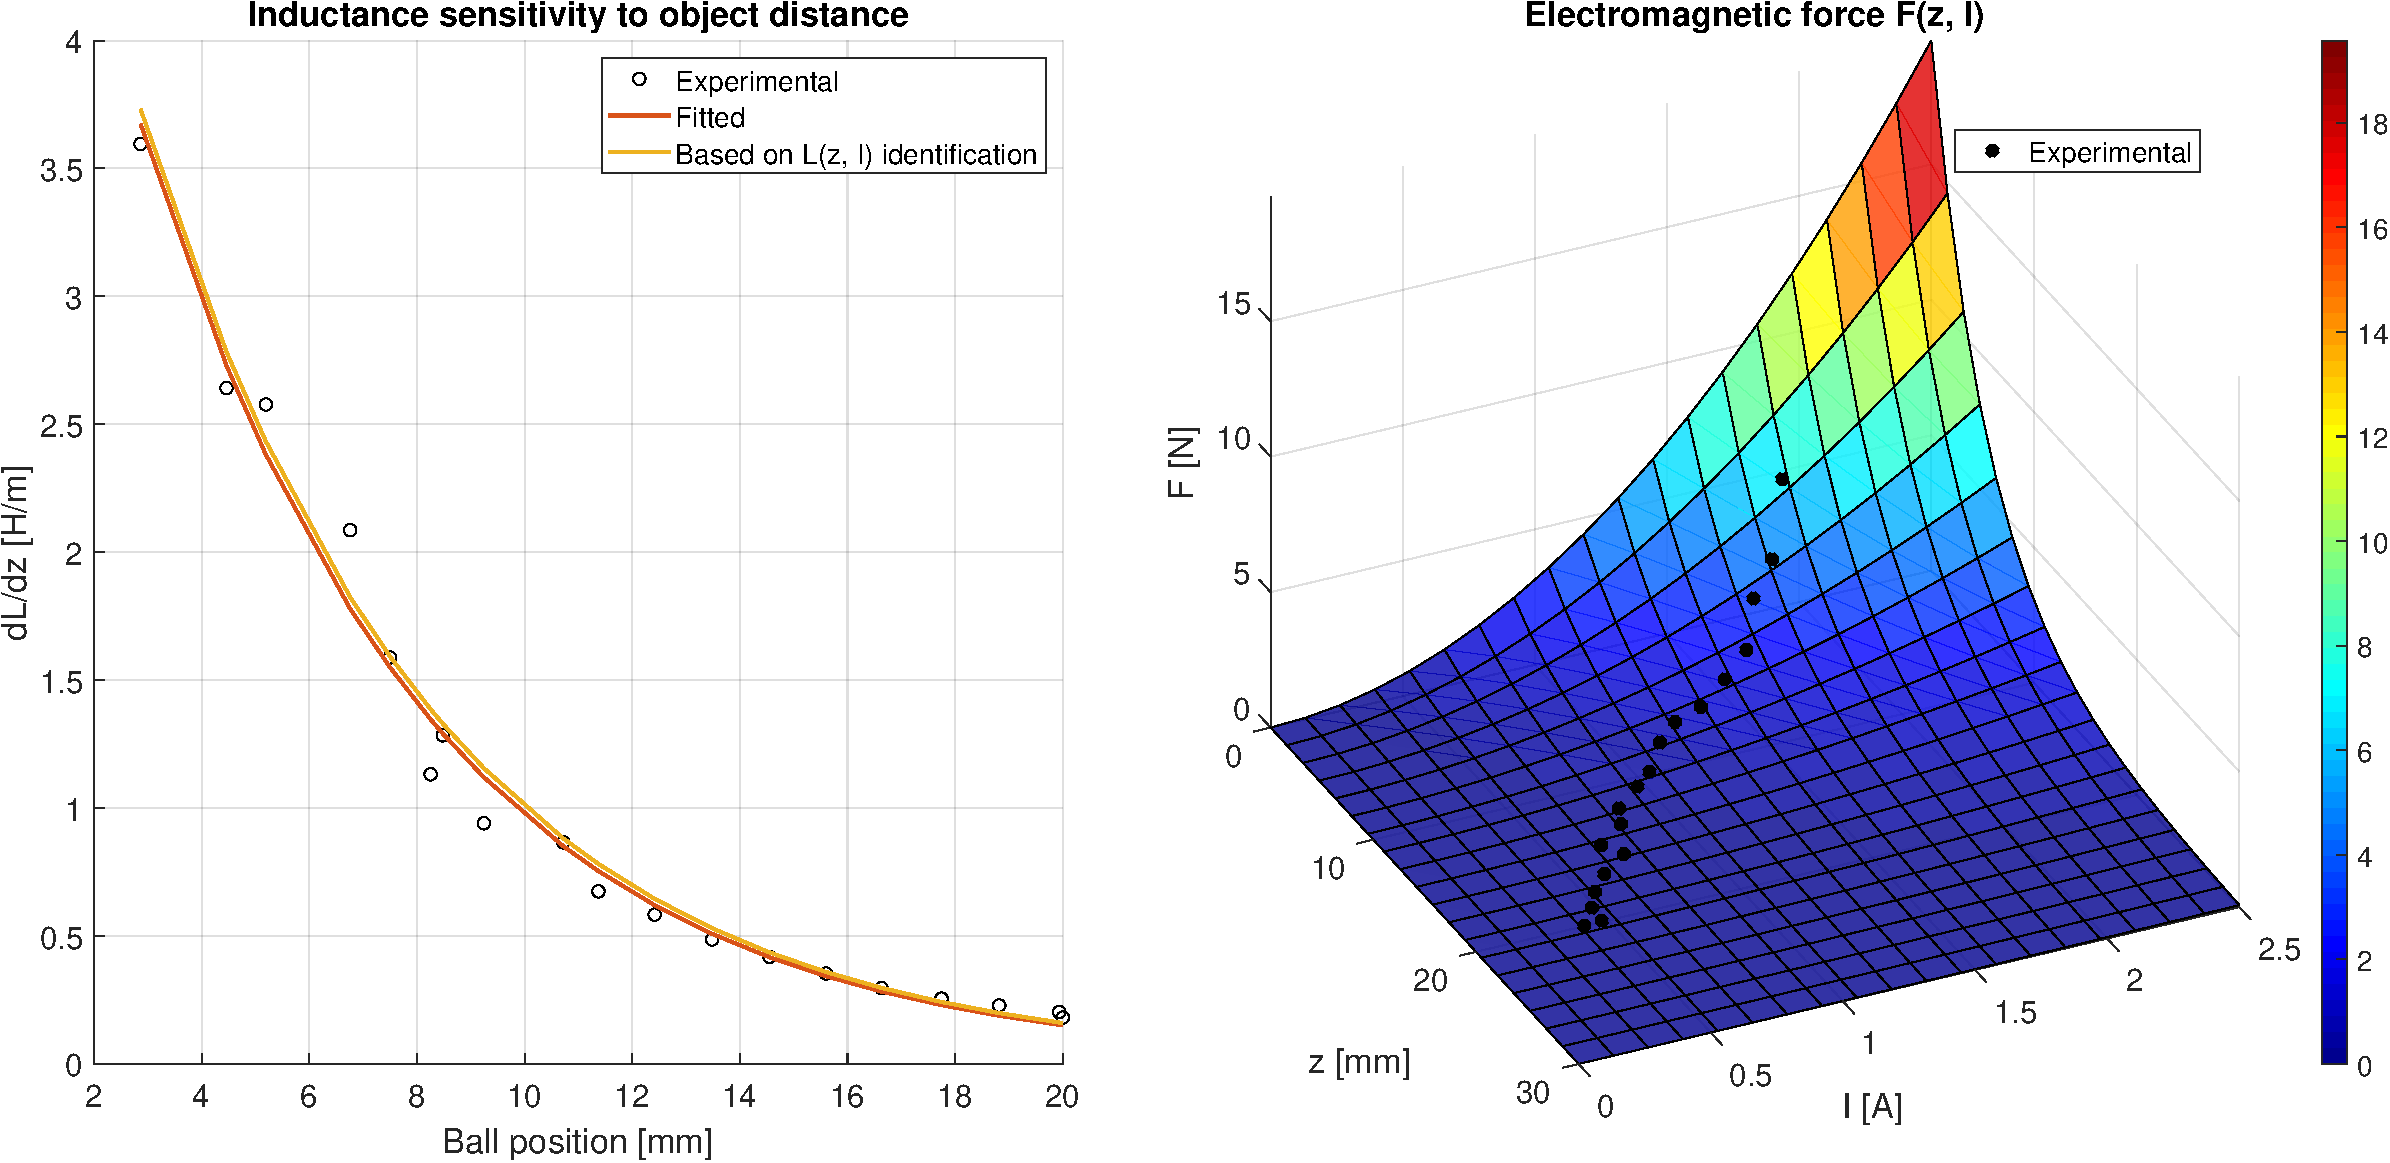
\includegraphics[width=1\textwidth]{img/MATLAB/identification/force.pdf}
            % \caption{Electromagnetic force as a function of $z$ and $I$}
        \end{figure}

        As a subsequent result, a complete model for the electromagnetic force is also obtained.

    }

\end{frame}



\begin{frame}{Identified parameters}

    All the identified parameters are listed in the following tables:

    \begin{table}[H]
        \centering
        \begin{tabular}{|c|l|c||c|l|c|}
            \hline
            \textbf{Parameter} & \textbf{Value}        & \textbf{Unit} & \textbf{Parameter} & \textbf{Value}       & \textbf{Unit} \\
            \hline
            $m$                & $60.54 \cdot 10^{-3}$ & kg            & $L_{0}$            & $6.54 \cdot 10^{-2}$ & H             \\
            $V_{min}$          & $4.30 \cdot 10^{-2}$  & V             & $a_{z}$            & $1.59 \cdot 10^{2}$  & 1/m           \\
            $U_{min}$          & $5.18 \cdot 10^{-2}$  & MU            & $L_{z}$            & $4.04 \cdot 10^{-2}$ & H             \\
            $k$                & $1.16 \cdot 10^{1}$   & V/MU          & $a_{I}$            & $5.30$               & -             \\
            $c$                & $-5.60 \cdot 10^{-1}$ & V             & $b_{I}$            & $1.04$               & A             \\
            $R_{0}$            & $4.17$                & $\Omega$      & $L_{I}$            & $3.29 \cdot 10^{-2}$ & H             \\
            \hline
        \end{tabular}

        \caption{Model's identified parameters}
    \end{table}

    \begin{table}[H]
        \centering

        \begin{tabular}{|c|c|c|}
            \hline
            \textbf{Sensor} & \textbf{Standard deviation}    & \textbf{Covariance}               \\
            \hline
            Infrared        & $2.68 \cdot 10^{-5} \quad [m]$ & $7.21 \cdot 10^{-10} \quad [m^2]$ \\
            Current         & $6.48 \cdot 10^{-3} \quad [A]$ & $4.21 \cdot 10^{-5} \quad [A^2]$  \\
            \hline
        \end{tabular}

        \caption{Sensors' noise parameters.}
    \end{table}

    \footnotetext{MU stands for `Machine Unit'}

\end{frame}